\chapter{Voronoi-Diagramme und Delaunay-Triangulation}
\label{chap:voronoi}

\begin{itemize*}
\item Was ist eine Delaunay-Triangulation?
\item Was ist ein Voronoi-Diagramm?
\item Wozu brauche ich Voronoi-Diagramme?
	\begin{itemize*}
	\item Dateisuche
	\item Collision Detection
	\end{itemize*}
\item Wie kann ich sie erzeugen?
	\begin{itemize*}
	\item Verbindungslinen zwischen den Knoten
	\item Lot auf den Mittelpunkt der VL
	\item Schnittpunkte der Lote
	\item Verbindungslinien der Schnittpunkte
	\end{itemize*}
	\begin{itemize*}
	\item Sweepline Algorithmus \cite{Fortune1987}
	\item Über Delaunay-Triangulation \cite{Dwyer1987}
	\end{itemize*}
	
\end{itemize*}

\begin{figure}[htbp]
\centering
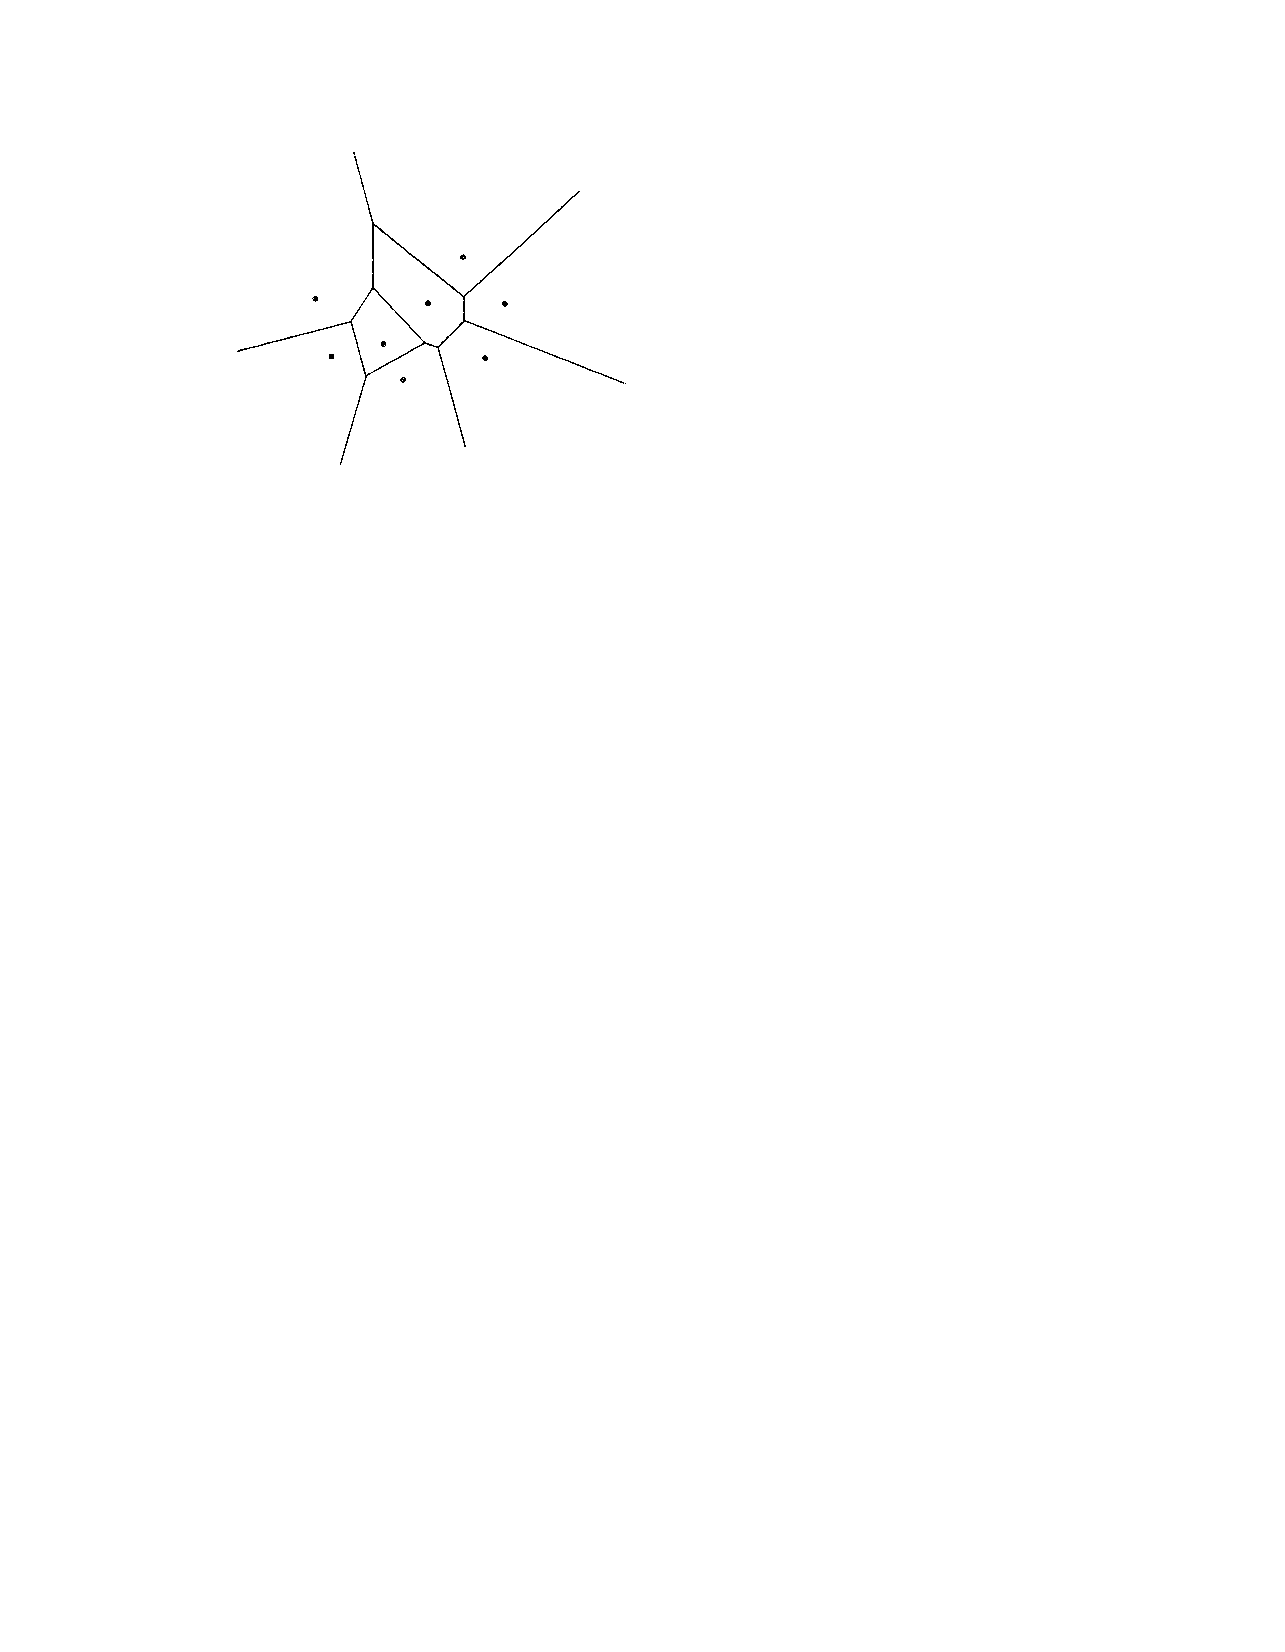
\includegraphics{grafics/voronoi_grund_aus_aurenhammer.pdf}
\caption{Voronoi-Diagramm für acht Punkte (aus \cite{Aurenhammer1991Voronoi})}
\label{fig:voronoi_grund}
\end{figure}





\begin{figure}[htbp]
\centering
\subfigure[Dualität von Voronoi-Diagramm und De\-launay-Triangulation (aus \cite{Aurenhammer1991Voronoi})]{
	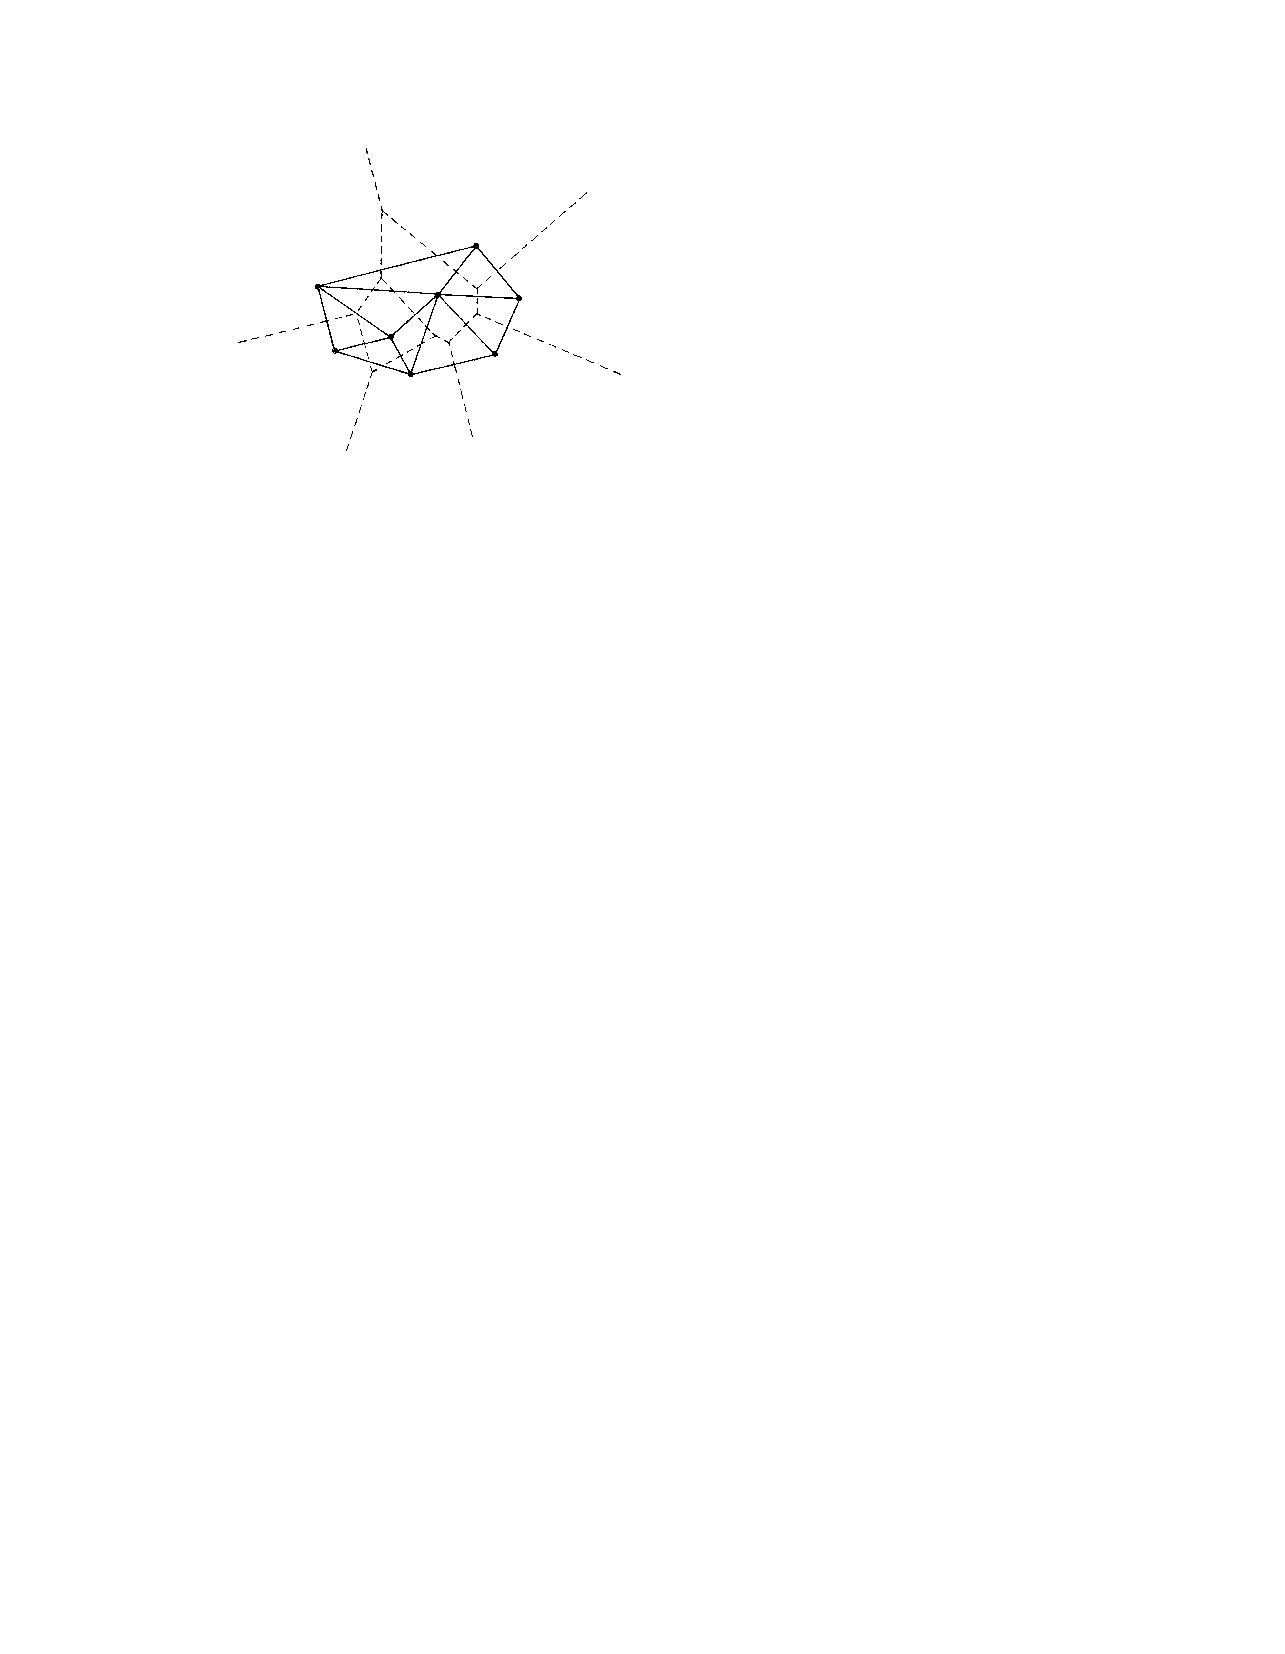
\includegraphics{grafics/voronoi_dual_aus_aurenhammer.pdf}
	\label{fig:voronoi_dual}
}
\subfigure[Bezug eines Voronoi-Diagrammes zur konvexen Hülle (aus \cite{Aurenhammer1991Voronoi})]{
	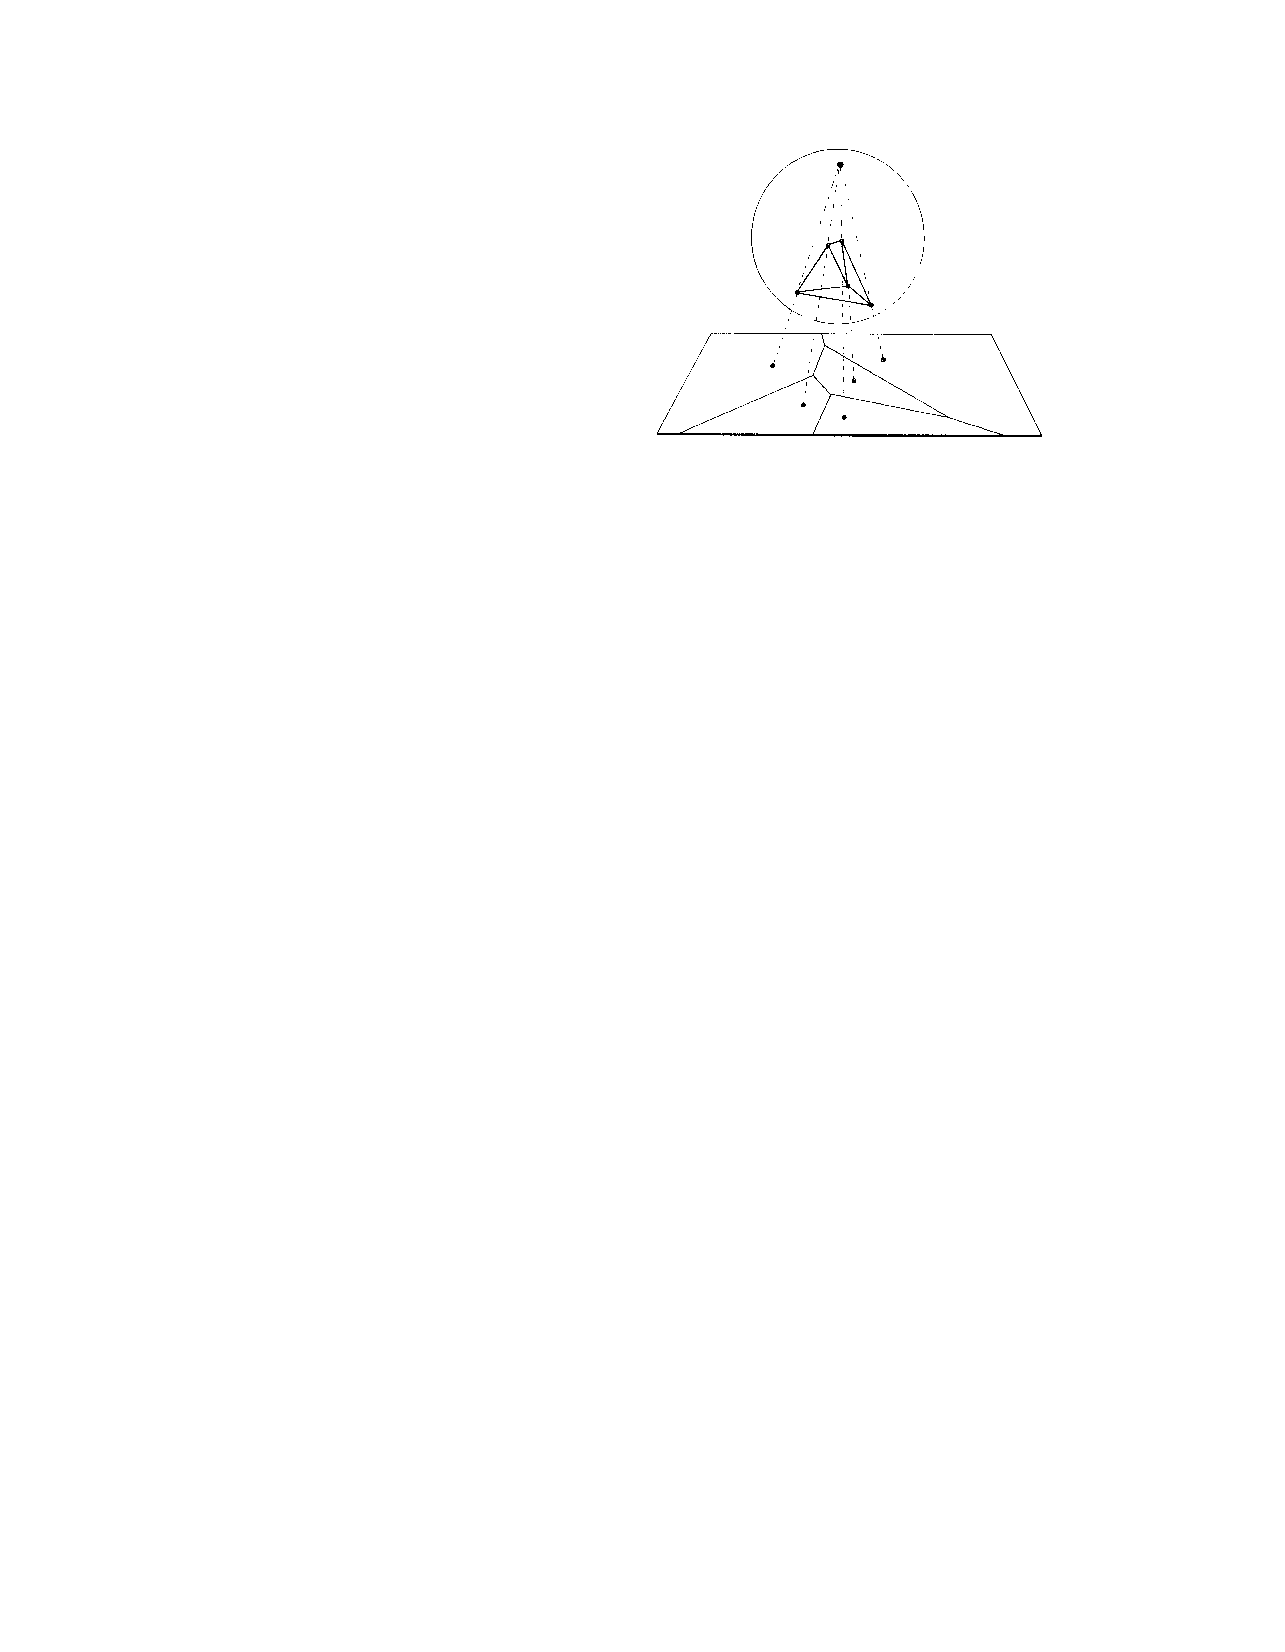
\includegraphics{grafics/voronoi_konvex_aus_aurenhammer.pdf}
	\label{fig:voronoi_konvex}
}
\end{figure}

\cite{Aurenhammer1991Voronoi}

\cite{Fortune1987, Dwyer1987} %Erzeugen von Voronoi-Diagrammen (Sweepline und Co)
